\documentclass[letterpaper,12pt]{article}
\usepackage[top=3.0cm, bottom=3.0cm, left=3.0cm, right=3.0cm]{geometry}
\usepackage[spanish]{babel}
\spanishdecimal{.}
\selectlanguage{spanish}
\usepackage[spanish,onelanguage,ruled]{algorithm2e}
\usepackage[utf8]{inputenc}
\usepackage{graphicx}
\usepackage{caption}
\usepackage{subcaption}
\usepackage{hyperref}
\usepackage{verbatim}
\usepackage{amssymb}
\usepackage{mathtools}
\usepackage{amsmath}
\usepackage[natbibapa]{apacite}
\bibliographystyle{apacite}
%\usepackage[nottoc,numbib]{tocbibind}
\newcommand\ddfrac[2]{\frac{\displaystyle #1}{\displaystyle #2}}
\DeclareMathOperator{\atantwo}{atan2}
\title{AutoModelCar League\\Mexican Robotics Tournament}
\author{Rulebook - Virtual modality}
\date{Ciudad Victoria, Tamaulipas, 2022}

\begin{document}
\renewcommand{\tablename}{Tabla}
\maketitle

%%%%%%%%%%%%%%%%%%%%%%%%%%%%%%%%%%%%%%%
%%%%%%%%% AGRADECIMIENTOS %%%%%%%%%%%%%
%%%%%%%%%%%%%%%%%%%%%%%%%%%%%%%%%%%%%%%
\section*{Acknowledgement}
This competition started thanks to the project ``Visiones de Movilidad Urbuna'', under direction of Prof. Raul Rojas of the Freie Universität Berlin. With this project, 32 scaled vehicles were donated to several universities, institutes and research centers in Mexico. Due to the pandemic and lockdown, in 2021 was held, by first time, the virtual modality of this competition, using the simulator developed by Dr. Marco Morales and his team, at Autonomous  Technological Institute of Mexico. On behalf of all beneficiary teams, we thank to all people that have contributed to the achievement of this competition.

\begin{flushright}
  \textit{
  The technical committe\\
  April, 2022
  }
\end{flushright}

\section{Introduction}
The Mexican Robotics Tournament (TMR by its spanish acronym) is the most important robotics competition in Mexico which year after year gathers students, teachers and researchers. Its main goal is to foster research and development of robotics in Mexico. Keeping this in mind, the TMR includes different competition leagues where participating teams can test their knowledge and capabilities in robotics.

For the second time, we open the simulated modality of the self-driving cars category where we propose several autonomous driving tasks. In the first edition, we used the simulator developed to model the scaled vehicles AutoNOMOS, donated by the Free University of Berlin. This year, we will use the Webots simulator with the objective of having more realistic vehicles and environments.

The direct predecessor of this rulebook are the event held in april, 2017, in the National Politechnic Institute, in Mexico City, and the previous editions of the AutoModelCar league of the Mexican Robotics Tournament. The present document aims to reuse the proposed tests with minimum adaptations and to stablish competition criteria to strengthen academic and student participation, as well as the exchange of experiences for development and training of professionals in this area of knowledge. 

%%%%%%%%%%%%%%%%%%%%%%%%%%%%%%%%%%%%%%%
%%%%%%%% SIMULATED VEHICLE %%%%%%%%%%
%%%%%%%%%%%%%%%%%%%%%%%%%%%%%%%%%%%%%%%
\section{About the simulated vehicle}
The simulator to be used is Webots\footnote{https://cyberbotics.com/doc/automobile/index} and the vehicle will be the model BMX X5\footnote{https://www.cyberbotics.com/doc/automobile/car?version=master} included in the default models of such simulator. Figure \ref{fig:BmwX5} shows a view of BMX X5 vehicle in the simulated environment. This vehicle is equipped with the following sensors:
\begin{enumerate}
\item RGB 640x480 camera with 3\% of noise. The camera is mounted on the top of the vehicle's windshield. 
\item 3D lidar sensor with the following features:
  \begin{enumerate}
  \item Horizontal field of view:  $360\deg$
  \item Vertical field of view: $18\deg$
  \item Number of layers: 32
  \item Minimum distance: 0.01 m
  \item Maximum distance: 75 m
  \item Horizontal resolution: 360
  \item Other default features included in Webots simulator\footnote{https://cyberbotics.com/doc/reference/lidar}.
  \end{enumerate}
\item GPS with 2m resolution, 0.1m of noise and the rest of default features included in Webots simulator\footnote{https://cyberbotics.com/doc/reference/gps}
\item Gyroscope, with all default features included in Webots simulator\footnote{https://www.cyberbotics.com/doc/reference/gyro?version=master}
\end{enumerate}

The following signals are considered as control signals:
\begin{enumerate}
\item Linear speed, given in [m/s]
\item Front wheel steering, given in [rad]
\end{enumerate}
It is not necessary to control the vehicle through torques of forces. The simulated vehicle already includes a speed and steering control to reach the desired speed and steering.

\begin{figure}
  \centering
  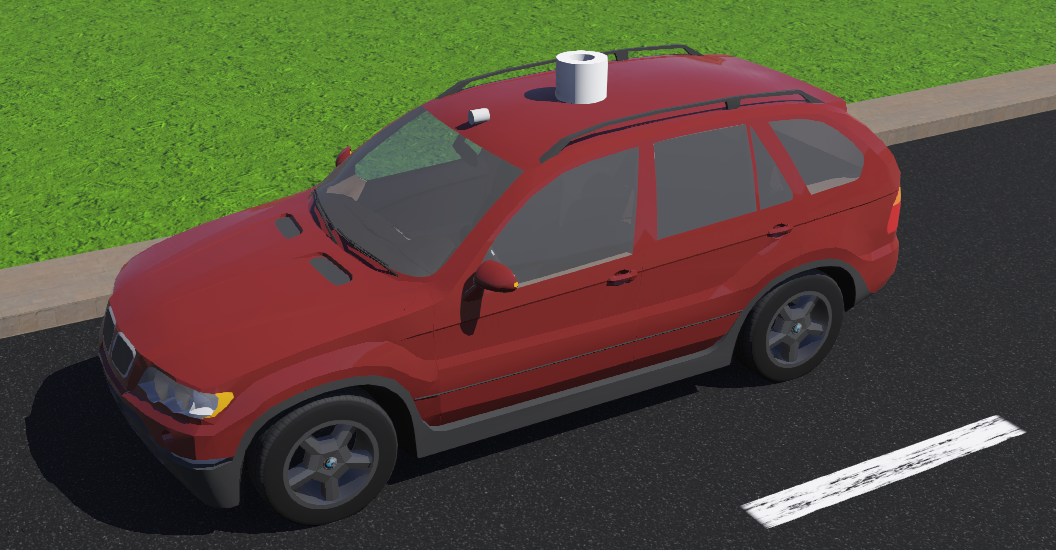
\includegraphics[width=0.75\textwidth]{Figures/Bmw.png}
  \caption{Simulated vehicle BMW X5}
  \label{fig:BmwX5}
\end{figure}

\subsection{ROS Integration}
The virtual modality aims to be as much similar as possible to the in-person modality. Keeping this in mind, the simulated vehicle interacts using the ROS platform in order to make developed software in simulation, also useful for real scaled vehicles, and viceversa. Therefore, the way to interact with the simulated vehicle is throught ROS publishers and subscribers. 

\begin{itemize}
\item Published topics:
  \begin{itemize}
  \item \texttt{/camera/rgb/raw} (sensor\_msgs/Image): RGB Camera image
  \item \texttt{/point\_cloud} (sensor\_msgs/PointCloud2): Point cloud generated by the 3D lidar
  \item \texttt{/gps} (sensor\_msgs/NavSatFix): GPS readings
  \item \texttt{/gyro} (sensor\_msgs/Imu): Gyro readings
  \end{itemize}
\item Subscribed topics:
  \begin{itemize}
  \item \texttt{/speed} (std\_msgs/Float64): Goal linear speed [m/s]
  \item \texttt{/steering} (std\_msgs/Float64): Goal steering [rad]
  \end{itemize}
\end{itemize}
\end{document}